\invisiblesection{Appendix C: Written Questioning of Donald J. Trump}

\thispagestyle{empty}

\vspace*{15em}

\begin{center}

\Huge
Appendix C

\end{center}

\newpage

\subsection{Introductory Note}

The President provided written responses through his personal counsel to questions submitted to him by the Special Counsel's Office. We first explain the process that led to the submission of written questions and then attach the President's responses.

Beginning in December 2017, this Office sought for more than a year to interview the President on topics relevant to both Russian-election interference and obstruction-of-justice.
We advised counsel that the President was a ``subject'' of the investigation under the definition of the Justice Manual---``a person whose conduct is within the scope of the grand jury's investigation.''
Justice Manual \S~9-11.151 (2018).
We also advised counsel that ``[a]n interview with the President is vital to our investigation'' and that this Office had ``carefully considered the constitutional and other arguments raised by \dots\ counsel, and they d[id] not provide us with reason to forgo seeking an interview.''% 1
\footnote{5/16/18 Letter, Special Counsel to the President's Personal Counsel, at~1.}
We additionally stated that ``it is in the interest of the Presidency and the public for an interview to take place'' and offered ``numerous accommodations to aid the President's preparation and avoid surprise.''% 2
\footnote{5/16/18 Letter, Special Counsels's Office to the President's Personal Counsel, at~1;
\textit{see} 7/30/18 Letter, Special Counsel's Office to the President's Personal Counsel, at~1 (describing accommodations).}
After extensive discussions with the Department of Justice about the Special Counsel's objective of securing the President's testimony, these accommodations included the submissions of written questions to the President on certain Russia-related topics.% 3
\footnote{9/17/18 Letter, Special Counsel's Office to the President's Personal Counsel, at~1 (submitting written questions).}

We received the President's written responses in late November 2018.% 4
\footnote{11/20/18 Letter, President's Personal Counsel to the Special Counsel's Office (transmitting written responses of Donald J. Trump).}
In December 2018, we informed counsel of the insufficiency of those responses in several respects.% 5
\footnote{12/3/18 Letter, Special Counsel's Office to the President's Personal Counsel, at~3.}
We noted, among other things, that the President stated on more than 30 occasions that he ``does not `recall' or `remember' or have an `independent recollection'{}'' of information called for by the questions.% 6
\footnote{12/3/18 Letter, Special Counsel's Office to the President's Personal Counsel, at~3.}
Other answers were ``incomplete or imprecise.''% 7
\footnote{12/3/18 Letter, Special Counsel's Office to the President's Personal Counsel, at~3;
\textit{see} (noting, ``for example,'' that the President ``did not answer whether he had at any time directed or suggested that discussions about the Trump Moscow Project should cease \dots\ but he has since made public comments about that topic'').}
The written responses, we informed counsel, ``demonstrate the inadequacy of the written format, as we have had no opportunity to ask follow-up questions that would ensure complete answers and potentially refresh your client's recollection or clarify the extent or nature of his lack of recollection.''% 8
\footnote{12/3/18 Letter, Special Counsel's Office to the President's Personal Counsel, at~3.}
We again requested an in-person interview, limited to certain topics, advising the President's counsel that ``[t]his is the President's opportunity to voluntarily provide us with information for us to evaluate in the context of all of the evidence we have gathered.''% 9
\footnote{12/3/18 Letter, Special Counsel to the President's Personal Counsel.}
The President declined.% 10
\footnote{12/12/18 Letter, President's Personal Counsel to the Special Counsel's Office, at~2.}

\blackout{Grand Jury}% 11
\footnote{\blackout{Grand Jury}}
\blackout{Grand Jury}% 12
\footnote{\blackout{Grand Jury}}

Recognizing that the President would not be interviewed voluntarily, we considered whether to issue a subpoena for his testimony.
We viewed the written answers to be inadequate.
But at that point, our investigation had made significant progress and had produced substantial evidence for our report.
We thus weighed the costs of potentially lengthy constitutional litigation, with resulting delay in finishing our investigation, against the anticipated benefits for our investigation and report.
As explained in Volume~II, Section II.B., we determined that the substantial quantity of information we had obtained from other sources allowed us to draw relevant factual conclusions on intent and credibility, which are often inferred from circumstantial evidence and assessed without direct testimony from the subject of the investigation.

\hr

\newpage

\subsection{WRITTEN QUESTIONS TO BE ANSWERED UNDER OATH BY PRESIDENT DONALD J. TRUMP}

\subsubsection{June 9, 2016 Meeting at Trump Tower}

\begin{enumerate}[a.]

\item When did you first learn that Donald Trump, Jr., Paul Manafort, or Jared Kushner was considering participating in a meeting in June 2016 concerning potentially negative information about Hillary Clinton?
Describe who you learned the information from and the substance of the discussion.

\item Attached to this document as Exhibit A is a series of emails from June 2016 between, among others, Donald Trump, Jr.\ and Rob Goldstone.
In addition to the emails reflected in Exhibit A, Donald Trump, Jr.\ had other communications with Rob Goldstone and Emin Agalarov between June 3, 2016, and June 9, 2016.

\begin{enumerate}[i.]

\item Did Mr.~Trump, Jr.\ or anyone else tell you about or show you any of these communications?
If yes, describe who discussed the communications with you, when, and the substance of the discussion(s).

\item When did you first see or learn about all or any part of the emails reflected in Exhibit A?

\item When did you first learn that the proposed meeting involved or was described as being part of Russia and its government's support for your candidacy?

\item Did you suggest to or direct anyone not to discuss or release publicly all or any portion of the emails reflected in Exhibit A? If yes, describe who you communicated with, when, the substance of the communication(s), and why you took that action.

\end{enumerate}

\item On June 9, 2016, Donald Trump, Jr., Paul Manafort, and Jared Kushner attended a meeting at Trump Tower with several individuals, including a Russian lawyer, Natalia Veselnitskaya (the ``June 9 meeting'').

\begin{enumerate}[i.]

\item Other than as set forth in your answers to 1.a and 1.b, what, if anything, were you told about the possibility of this meeting taking place, or the scheduling of such a meeting?
Describe who you discussed this with, when, and what you were informed about the meeting.

\item When did you learn that some of the individuals attending the June 9 meeting were Russian or had any affiliation with any part of the Russian government?
Describe who you learned this information from and the substance of the discussion(s).

\item What were you told about what was discussed at the June 9 meeting?
Describe each conversation in which you were told about what was discussed at the meeting, who the conversation was with, when it occurred, and the substance of the statements they made about the meeting.

\item Were you told that the June 9 meeting was about, in whole or in part, adoption and/or the Magnitsky Act?
If yes, describe who you had that discussion with, when, and the substance of the discussion.

\end{enumerate}

\item For the period June 6, 2016 through June 9, 2016, for what portion of each day were you in Trump Tower?

\begin{enumerate}[i.]

\item Did you speak or meet with Donald Trump, Jr., Paul Manafort, or Jared Kushner on June 9, 2016?
If yes, did any portion of any of those conversations or meetings include any reference to any aspect of the June 9 meeting?
If yes, describe who you spoke with and the substance of the conversation.

\end{enumerate}

\item Did you communicate directly or indirectly with any member or representative of the Agalarov family after June 3, 2016?
If yes, describe who you spoke with, when, and the substance of the communication.

\item Did you learn of any communications between Donald Trump, Jr., Paul Manafort, or Jared Kushner and any member or representative of the Agalarov family, Natalia Veselnitskaya, Rob Goldstone, or any Russian official or contact that took place after June 9, 2016 and concerned the June 9 meeting or efforts by Russia to assist the campaign?
If yes, describe who you learned this information from, when, and the substance of what you learned.

\item On June 7, 2016, you gave a speech in which you said, in part, ``I am going to give a major speech on probably Monday of next week and we're going to be discussing all of the things that have taken place with the Clintons.''

\begin{enumerate}[i.]

\item Why did you make that statement?
\item What information did you plan to share with respect to the Clintons?
\item What did you believe the source(s) of that information would be?
\item Did you expect any of the information to have come from the June 9 meeting?
\item Did anyone help draft the speech that you were referring to? If so, who?
\item Why did you ultimately not give the speech you referenced on June 7, 2016?

\end{enumerate}

\item Did any person or entity inform you during the campaign that Vladimir Putin or the Russian government supported your candidacy or opposed the candidacy of Hillary Clinton?
If yes, describe the source(s) of the information, when you were informed, and the content of such discussion(s).

\item Did any person or entity inform you during the campaign that any foreign government or foreign leader, other than Russia or Vladimir Putin, had provided, wished to provide, or offered to provide tangible support to your campaign, including by way of offering to provide negative information on Hillary Clinton?
If yes, describe the source(s) of the information, when you were informed, and the content of such discussion(s).

\end{enumerate}

\subsubsection{Russian Hacking / Russian Efforts Using Social Media / Wikileaks}

\begin{enumerate}[a.]

\item On June 14, 2016, it was publicly reported that computer hackers had penetrated the computer network of the Democratic National Committee (DNC) and that Russian intelligence was behind the unauthorized access, or hack.
Prior to June 14, 2016, were you provided any information about any potential or actual hacking of the computer systems or email accounts of the DNC, the Democratic Congressional Campaign Committee (DCCC), the Clinton Campaign, Hillary Clinton, or individuals associated with the Clinton campaign?
If yes, describe who provided this information, when, and the substance of the information.

\item On July 22, 2016, WikiLeaks released nearly 20,000 emails sent or received by Democratic party officials.

\begin{enumerate}[i.]

\item Prior to the July 22, 2016 release, were you aware from any source that WikiLeaks, Guccifer~2.0, DCLeaks, or Russians had or potentially had possession of or planned to release emails or information that could help your campaign or hurt the Clinton campaign?
If yes, describe who you discussed this issue with, when, and the substance of the discussion(s).

\item After the release of emails by WikiLeaks on July 22, 2016, were you told that WikiLeaks possessed or might possess additional information that could be released during the campaign?
If yes, describe who provided this information, when, and what you were told.

\end{enumerate}

\item Are you aware of any communications during the campaign, directly or indirectly, between Roger Stone, Donald Trump, Jr., Paul Manafort, or Rick Gates and (a)~WikiLeaks, (b)~Julian Assange, (c)~other representatives of WikiLeaks, (d)~Guccifer~2.0, (e)~representatives of Guccifer~2.0, or (f)~representatives of DCLeaks?
If yes, describe who provided you with this information, when you learned of the communications, and what you know about those communications.

\item On July 27, 2016, you stated at a press conference: ``Russia, if you're listening, I hope you're able to find the 30,000 emails that are missing.
I think you will probably be rewarded mightily by our press.''

\begin{enumerate}[i.]

\item Why did you make that request of Russia, as opposed to any other country, entity, or individual?

\item In advance of making that statement, what discussions, if any, did you have with anyone else about the substance of the statement?

\item Were you told at any time before or after you made that statement that Russia was attempting to infiltrate or hack computer systems or email accounts of Hillary Clinton or her campaign?
If yes, describe who provided this information, when, and what you were told.

\end{enumerate}

\item On October 7, 2016, emails hacked from the account of John Podesta were released by WikiLeaks.

\begin{enumerate}[i.]

\item Where were you on October 7, 2016?

\item Were you told at any time in advance of, or on the day of, the October 7 release that WikiLeaks possessed or might possess emails related to John Podesta?
If yes, describe who told you this, when, and what you were told.

\item Are you aware of anyone associated with you or your campaign, including Roger Stone, reaching out to WikiLeaks, either directly or through an intermediary, on or about October 7, 2016?
If yes, identify the person and describe the substance of the conversations or contacts.

\end{enumerate}

\item Were you told of anyone associated with you or your campaign, including Roger Stone, having any discussions, directly or indirectly, with WikiLeaks, Guccifer~2.0, or DCLeaks regarding the content or timing of release of hacked emails?
If yes, describe who had such contacts, how you became aware of the contacts, when you became aware of the contacts, and the substance of the contacts.

\item From June 1, 2016 through the end of the campaign, how frequently did you communicate with Roger Stone? Describe the nature of your communication(s) with Mr.~Stone.

\begin{enumerate}[i.]

\item During that time period, what efforts did Mr.~Stone tell you he was making to assist your campaign, and what requests, if any, did you make of Mr.~Stone?

\item Did Mr.~Stone ever discuss WikiLeaks with you or, as far as you were aware, with anyone else associated with the campaign?
If yes, describe what you were told, from whom, and when.

\item Did Mr.~Stone at any time inform you about contacts he had with WikiLeaks or any intermediary of Wikileaks, or about forthcoming releases of information?
If yes, describe what Stone told you and when.

\end{enumerate}

\item Did you have any discussions prior to January 20, 2017, regarding a potential pardon or other action to benefit Julian Assange?
If yes, describe who you had the discussion(s) with, when, and the content of the discussion(s).

\item Were you aware of any efforts by foreign individuals or companies, including those in Russia, to assist your campaign through the use of social media postings or the organization of rallies?
If yes, identify who you discussed such assistance with, when, and the content of the discussion(s).

\end{enumerate}

\subsubsection{The Trump Organization Moscow Project}

\begin{enumerate}[a.]

\item In October 2015, a ``Letter of Intent,'' a copy of which is attached as Exhibit B, was signed for a proposed Trump Organization project in Moscow (the ``Trump Moscow project'').

\begin{enumerate}[i.]

\item When were you first informed of discussions about the Trump Moscow project?
By whom?
What were you told about the project?

\item Did you sign the letter of intent?

\end{enumerate}

\item In a statement provided to Congress, attached as Exhibit C, Michael Cohen stated: ``To the best of my knowledge, Mr.~Trump was never in contact with anyone about this proposal other than me on three occasions, including signing a non-binding letter of intent in 2015.''
Describe all discussions you had with Mr.~Cohen, or anyone else associated with the Trump Organization, about the Trump Moscow project, including who you spoke with, when, and the substance of the discussion(s).

\item Did you learn of any communications between Michael Cohen or Felix Sater and any Russian government officials, including officials in the office of Dmitry Peskov, regarding the Trump Moscow project?
If so, identify who provided this information to you, when, and the substance of what you learned.

\item Did you have any discussions between June 2015 and June 2016 regarding a potential trip to Russia by you and/or Michael Cohen for reasons related to the Trump Moscow project?
If yes, describe who you spoke with, when, and the substance of the discussion(s).

\item Did you at any time direct or suggest that discussions about the Trump Moscow project should cease, or were you informed at any time that the project had been abandoned?
If yes, describe who you spoke with, when, the substance of the discussion(s), and why that decision was made.

\item Did you have any discussions regarding what information would be provided publicly or in response to investigative inquiries about potential or actual investments or business deals the Trump Organization had in Russia, including the Trump Moscow project?
If yes, describe who you spoke with, when, and the substance of the discussion(s).

\item Aside from the Trump Moscow project, did you or the Trump Organization have any other prospective or actual business interests, investments, or arrangements with Russia or any Russian interest or Russian individual during the campaign?
If yes, describe the business interests, investments, or arrangements.

\end{enumerate}

\subsubsection{Contacts with Russia and Russia-Related Issues During the Campaign}

\begin{enumerate}[a.]

\item Prior to mid-August 2016, did you become aware that Paul Manafort had ties to the Ukrainian government?
If yes, describe who you learned this information from, when, and the substance of what you were told.
Did Mr.~Manafort's connections to the Ukrainian or Russian governments play any role in your decision to have him join your campaign?
If yes, describe that role.

\item Were you aware that Paul Manafort offered briefings on the progress of your campaign to Oleg Deripaska?
If yes, describe who you learned this information from, when, the substance of what you were told, what you understood the purpose was of sharing such information with Mr.~Deripaska, and how you responded to learning this information.

\item Were you aware of whether Paul Manafort or anyone else associated with your campaign sent or directed others to send internal Trump campaign information to any person located in Ukraine or Russia or associated with the Ukrainian or Russian governments?
If yes, identify who provided you with this information, when, the substance of the discussion(s), what you understood the purpose was of sharing the internal campaign information, and how you responded to learning this information.

\item Did Paul Manafort communicate to you, directly or indirectly, any positions Ukraine or Russia would want the U.S. to support?
If yes, describe when he communicated those positions to you and the substance of those communications.

\item During the campaign, were you told about efforts by Russian officials to meet with you or senior members of your campaign?
If yes, describe who you had conversations with on this topic, when, and what you were told.

\item What role, if any, did you have in changing the Republican Party platform regarding arming Ukraine during the Republican National Convention?
Prior to the convention, what information did you have about this platform provision?
After the platform provision was changed, who told you about the change, when did they tell you, what were you told about why it was changed, and who was involved?

\item On July 27, 2016, in response to a question about whether you would recognize Crimea as Russian territory and lift sanctions on Russia, you said: ``We'll be looking at that. Yeah, we'll be looking.''
Did you intend to communicate by that statement or at any other time during the campaign a willingness to lift sanctions and/or recognize Russia's annexation of Crimea if you were elected?

\begin{enumerate}[i.]

\item What consideration did you give to lifting sanctions and/or recognizing Russia's annexation of Crimea if you were elected?
Describe who you spoke with about this topic, when, the substance of the discussion(s).

\end{enumerate}

\end{enumerate}

\subsubsection{Contacts with Russia and Russia-Related Issues During the Transition}

\begin{enumerate}[a.]

\item Were you asked to attend the World Chess Championship gala on November 10, 2016?
If yes, who asked you to attend, when were you asked, and what were you told about about why your presence was requested?

\begin{enumerate}[i.]

\item Did you attend any part of the event?
If yes, describe any interactions you had with any Russians or representatives of the Russian government at the event.

\end{enumerate}

\item Following the Obama Administration's imposition of sanctions on Russia in December 2016 (``Russia sanctions''), did you discuss with Lieutenant General (LTG) Michael Flynn, K.T. McFarland, Steve Bannon, Reince Priebus, Jared Kushner, Erik Prince, or anyone else associated with the transition what should be communicated to the Russian government regarding the sanctions?
If yes, describe who you spoke with about this issue, when, and the substance of the discussion(s).

\item On December 29 and December 31, 2016, LTG Flynn had conversations with Russian Ambassador Sergey Kislyak about the Russia sanctions and Russia's response to the Russia sanctions.

\begin{enumerate}[i.]

\item Did you direct or suggest that LTG Flynn have discussions with anyone from the Russian government about the Russia sanctions?

\item Were you told in advance of LTG Flynn's December 29, 2016 conversation that he was going to be speaking with Ambassador Kislyak?
If yes, describe who told you this information, when, and what you were told.
If no, when and from whom did you learn of LTG Flynn's December 29, 2016 conversation with Ambassador Kislyak?

\item When did you learn of LTG Flynn and Ambassador Kislyak's call on December 31, 2016? Who told you and what were you told?

\item When did you learn that sanctions were discussed in the December 29 and December 31, 2016 calls between LTG Flynn and Ambassador Kislyak?
Who told you and what were you told?

\end{enumerate}

\item At any time between December 31, 2016, and January 20, 2017, did anyone tell you or suggest to you that Russia's decision not to impose reciprocal sanctions was attributable in any way to LTG Flynn's communications with Ambassador Kislyak?
If yes, identify who provided you with this information, when, and the substance of what you were told.

\item On January 12, 2017, the Washington Post published a column that stated that LTG Flynn phoned Ambassador Kislyak several times on December 29, 2016.
After learning of the column, did you direct or suggest to anyone that LTG Flynn should deny that he discussed sanctions with Ambassador Kislyak?
If yes, who did you make this suggestion or direction to, when, what did you say, and why did you take this step?

\begin{enumerate}[i.]

\item After learning of the column, did you have any conversations with LTG Flynn about his conversations with Ambassador Kislyak in December 2016?
If yes, describe when those discussions occurred and the content of the discussions.

\end{enumerate}

\item Were you told about a meeting between Jared Kushner and Sergei Gorkov that took place in December 2016?

\begin{enumerate}[i.]

\item If yes, describe who you spoke with, when, the substance of the discussion(s), and what you understood was the purpose of the meeting.

\end{enumerate}

\item Were you told about a meeting or meetings between Erik Prince and Kirill Dmitriev or any other representative from the Russian government that took place in January 2017?

\begin{enumerate}[i.]

\item If yes, describe who you spoke with, when, the substance of the discussion(s), and what you understood was the purpose of the meeting(s).

\end{enumerate}

\item Prior to January 20, 2017, did you talk to Steve Bannon, Jared Kushner, or any other individual associated with the transition regarding establishing an unofficial line of communication with Russia?
If yes, describe who you spoke with, when, the substance of the discussion(s), and what you understood was the purpose of such an unofficial line of communication.

\end{enumerate}

\subsection{RESPONSES OF PRESIDENT DONALD J. TRUMP}

\subsubsection{June 9, 2016 Meeting at Trump Tower}

\begin{enumerate}[a.]

\item When did you first learn that Donald Trump, Jr., Paul Manafort, or Jared Kushner was considering participating in a meeting in June 2016 concerning potentially negative information about Hillary Clinton?
Describe who you learned the information from and the substance of the discussion.

\item Attached to this document as Exhibit A is a series of emails from June 2016 between, among others, Donald Trump, Jr.\ and Rob Goldstone.
In addition to the emails reflected in Exhibit A, Donald Trump, Jr.\ had other communications with Rob Goldstone and Emin Agalarov between June 3, 2016, and June 9, 2016.

\begin{enumerate}[i.]

\item Did Mr.~Trump, Jr.\ or anyone else tell you about or show you any of these communications?
If yes, describe who discussed the communications with you, when, and the substance of the discussion(s).

\item When did you first see or learn about all or any part of the emails reflected in Exhibit A?

\item When did you first learn that the proposed meeting involved or was described as being part of Russia and its government's support for your candidacy?

\item Did you suggest to or direct anyone not to discuss or release publicly all or any portion of the emails reflected in Exhibit A? If yes, describe who you communicated with, when, the substance of the communication(s), and why you took that action.

\end{enumerate}

\item On June 9, 2016, Donald Trump, Jr., Paul Manafort, and Jared Kushner attended a meeting at Trump Tower with several individuals, including a Russian lawyer, Natalia Veselnitskaya (the ``June 9 meeting'').

\begin{enumerate}[i.]

\item Other than as set forth in your answers to 1.a and 1.b, what, if anything, were you told about the possibility of this meeting taking place, or the scheduling of such a meeting?
Describe who you discussed this with, when, and what you were informed about the meeting.

\item When did you learn that some of the individuals attending the June 9 meeting were Russian or had any affiliation with any part of the Russian government?
Describe who you learned this information from and the substance of the discussion(s).

\item What were you told about what was discussed at the June 9 meeting?
Describe each conversation in which you were told about what was discussed at the meeting, who the conversation was with, when it occurred, and the substance of the statements they made about the meeting.

\item Were you told that the June 9 meeting was about, in whole or in part, adoption and/or the Magnitsky Act?
If yes, describe who you had that discussion with, when, and the substance of the discussion.

\end{enumerate}

\item For the period June 6, 2016 through June 9, 2016, for what portion of each day were you in Trump Tower?

\begin{enumerate}[i.]

\item Did you speak or meet with Donald Trump, Jr., Paul Manafort, or Jared Kushner on June 9, 2016?
If yes, did any portion of any of those conversations or meetings include any reference to any aspect of the June 9 meeting?
If yes, describe who you spoke with and the substance of the conversation.

\end{enumerate}

\item Did you communicate directly or indirectly with any member or representative of the Agalarov family after June 3, 2016?
If yes, describe who you spoke with, when, and the substance of the communication.

\item Did you learn of any communications between Donald Trump, Jr., Paul Manafort, or Jared Kushner and any member or representative of the Agalarov family, Natalia Veselnitskaya, Rob Goldstone, or any Russian official or contact that took place after June 9, 2016 and concerned the June 9 meeting or efforts by Russia to assist the campaign?
If yes, describe who you learned this information from, when, and the substance of what you learned.

\item On June 7, 2016, you gave a speech in which you said, in part, ``I am going to give a major speech on probably Monday of next week and we're going to be discussing all of the things that have taken place with the Clintons.''

\begin{enumerate}[i.]

\item Why did you make that statement?
\item What information did you plan to share with respect to the Clintons?
\item What did you believe the source(s) of that information would be?
\item Did you expect any of the information to have come from the June 9 meeting?
\item Did anyone help draft the speech that you were referring to? If so, who?
\item Why did you ultimately not give the speech you referenced on June 7, 2016?

\end{enumerate}

\item Did any person or entity inform you during the campaign that Vladimir Putin or the Russian government supported your candidacy or opposed the candidacy of Hillary Clinton?
If yes, describe the source(s) of the information, when you were informed, and the content of such discussion(s).

\item Did any person or entity inform you during the campaign that any foreign government or foreign leader, other than Russia or Vladimir Putin, had provided, wished to provide, or offered to provide tangible support to your campaign, including by way of offering to provide negative information on Hillary Clinton?
If yes, describe the source(s) of the information, when you were informed, and the content of such discussion(s).

\end{enumerate}

\paragraph*{Response to Question I, Parts (a) through (c)}

I have no recollection of learning at the time that Donald Trump, Jr., Paul Manafort, or Jared Kushner was considering participating in a meeting in June 2016 concerning potentially negative information about Hillary Clinton.
Nor do I recall learning during the campaign that the June 9, 2016 meeting had taken place, that the referenced emails existed, or that Donald J. Trump, Jr., had other communications with Emin Agalarov or Robert Goldstone between June 3, 2016 and June 9, 2016.

\paragraph*{Response to Question I, Part (d)}

I have no independent recollection of what portion of these four days in June of 2016 I spent in Trump Tower.
This was one of many busy months during a fast-paced campaign, as the primary season was ending and we were preparing for the general election campaign.

I am now aware that my Campaign's calendar indicates that I was in New York City from June 6 -9, 2016.
Calendars kept in my Trump Tower office reflect that I had various calls and meetings scheduled for each of these days.
While those calls and meetings may or may not actually have taken place, they do indicate that I was in Trump Tower during a portion of each of these working days, and I have no reason to doubt that I was.
When I was in New York City, I stayed at my Trump Tower apartment.

My Trump Organization desk calendar also reflects that I was outside Trump Tower during portions of these days.
The June 7, 2016 calendar indicates I was scheduled to leave Trump Tower in the early evening for Westchester where I gave remarks after winning the California, New Jersey, New Mexico, Montana, and South Dakota Republican primaries held that day.
The June 8, 2016 calendar indicates a scheduled departure in late afternoon to attend a ceremony at my son's school.
The June 9, 2016 calendar indicates I was scheduled to attend midday meetings and a fund raising luncheon at the Four Seasons Hotel.
At this point, I do not remember on what dates these events occurred, but I do not currently have a reason to doubt that they took place as scheduled on my calendar.

Widely available media reports, including television footage, also shed light on my activities during these days.
For example, I am aware that my June 7, 2016 victory remarks at the Trump National Golf Club in Briarcliff Manor, New York, were recorded and published by the media.
I remember winning those primaries and generally recall delivering remarks that evening.

At this point in time, I do not remember whether I spoke or met with Donald Trump, Jr., Paul Manafort, or Jared Kushner on June 9, 2016.
My desk calendar indicates I was scheduled to meet with Paul Manafort on the morning of June 9, but I do not recall if that meeting took place.
It was more than two years ago, at a time when I had many calls and interactions daily.

\paragraph*{Response to Question I, Part (e)}

I have no independent recollection of any communications I had with the Agalarov family or anyone I understood to be a representative of the Agalarov family after June 3, 2016 and before the end of the campaign.
While preparing to respond to these questions, I have become aware of written communications with the Agalarovs during the campaign that were sent, received, and largely authored by my staff and which I understand have already been produced to you.

In general, the documents include congratulatory letters on my campaign victories, emails about a painting Emin and Aras Agalarov arranged to have delivered to Trump Tower as a birthday present, and emails regarding delivery of a book written by Aras Agalarov.
The documents reflect that the deliveries were screened by the Secret Service.

\paragraph*{Response to Question I, Part (f)}

I do not recall being aware during the campaign of communications between Donald Trump, Jr., Paul Manafort, or Jared Kushner and any member or representative of the Agalarov family, Robert Goldstone, Natalia Veselnitskaya (whose name I was not familiar with), or anyone I understood to be a Russian official.

\paragraph*{Response to Question I, Part (g)}

In remarks I delivered the night I won the California, New Jersey, New Mexico, Montana, and South Dakota Republican primaries, I said, ``I am going to give a major speech on probably Monday of next week and we're going to be discussing all of the things that have taken place with the Clintons.''
In general, I expected to give a speech referencing the publicly available, negative information about the Clintons, including, for example, Mrs.~Clinton's failed policies, the Clintons' use of the State Department to further their interests and the interests of the Clinton Foundation, Mrs.~Clinton's improper use of a private server for State Department business, the destruction of 33,000 emails on that server, and Mrs.~Clinton's temperamental unsuitability for the office of President.

In the course of preparing to respond to your questions, I have become aware that the Campaign documents already produced to you reflect the drafting, evolution, and sources of information for the speech I expected to give ``probably'' on the Monday following my June 7, 2016 comments.
These documents generally show that the text of the speech was initially drafted by Campaign staff with input from various outside advisors and was based on publicly available material, including, in particular, information from the book Clinton Cash by Peter Schweizer.

The Pulse Nightclub terrorist attack took place in the early morning hours of Sunday, June 12, 2016.
In light of that tragedy, I gave a speech directed more specifically to national security and terrorism than to the Clintons.
That speech was delivered at the Saint Anselm College Institute of Politics in Manchester, New Hampshire, and, as reported, opened with the following:

\begin{quote}
This was going to be a speech on Hillary Clinton and how bad a President, especially in these times of Radical Islamic Terrorism, she would be.
Even her former Secret Service Agent, who has seen her under pressure and in times of stress, has stated that she lacks the temperament and integrity to be president.
There will be plenty of opportunity to discuss these important issues at a later time, and I will deliver that speech soon.
But today there is only one thing to discuss: the growing threat of terrorism inside of our borders.
\end{quote}

I continued to speak about Mrs.~Clinton's failings throughout the campaign, using the information prepared for inclusion in the speech to which I referred on June 7, 2016.

\paragraph*{Response to Question I, Part (h)}

I have no recollection of being told during the campaign that Vladimir Putin or the Russian government ``supported'' my candidacy or ``opposed'' the candidacy of Hillary Clinton.
However, I was aware of some reports indicating that President Putin had made complimentary statements about me.

\paragraph*{Response to Question I, Part (i)}

I have no recollection of being told during the campaign that any foreign government or foreign leader had provided, wished to provide, or offered to provide tangible support to my campaign.

\subsubsection{Russian Hacking / Russian Efforts Using Social Media / Wikileaks}

\begin{enumerate}[a.]

\item On June 14, 2016, it was publicly reported that computer hackers had penetrated the computer network of the Democratic National Committee (DNC) and that Russian intelligence was behind the unauthorized access, or hack.
Prior to June 14, 2016, were you provided any information about any potential or actual hacking of the computer systems or email accounts of the DNC, the Democratic Congressional Campaign Committee (DCCC), the Clinton Campaign, Hillary Clinton, or individuals associated with the Clinton campaign?
If yes, describe who provided this information, when, and the substance of the information.

\item On July 22, 2016, WikiLeaks released nearly 20,000 emails sent or received by Democratic party officials.

\begin{enumerate}[i.]

\item Prior to the July 22, 2016 release, were you aware from any source that WikiLeaks, Guccifer~2.0, DCLeaks, or Russians had or potentially had possession of or planned to release emails or information that could help your campaign or hurt the Clinton campaign?
If yes, describe who you discussed this issue with, when, and the substance of the discussion(s).

\item After the release of emails by WikiLeaks on July 22, 2016, were you told that WikiLeaks possessed or might possess additional information that could be released during the campaign?
If yes, describe who provided this information, when, and what you were told.

\end{enumerate}

\item Are you aware of any communications during the campaign, directly or indirectly, between Roger Stone, Donald Trump, Jr., Paul Manafort, or Rick Gates and (a)~WikiLeaks, (b)~Julian Assange, (c)~other representatives of WikiLeaks, (d)~Guccifer~2.0, (e)~representatives of Guccifer~2.0, or (f)~representatives of DCLeaks?
If yes, describe who provided you with this information, when you learned of the communications, and what you know about those communications.

\item On July 27, 2016, you stated at a press conference: ``Russia, if you're listening, I hope you're able to find the 30,000 emails that are missing.
I think you will probably be rewarded mightily by our press.''

\begin{enumerate}[i.]

\item Why did you make that request of Russia, as opposed to any other country, entity, or individual?

\item In advance of making that statement, what discussions, if any, did you have with anyone else about the substance of the statement?

\item Were you told at any time before or after you made that statement that Russia was attempting to infiltrate or hack computer systems or email accounts of Hillary Clinton or her campaign?
If yes, describe who provided this information, when, and what you were told.

\end{enumerate}

\item On October 7, 2016, emails hacked from the account of John Podesta were released by WikiLeaks.

\begin{enumerate}[i.]

\item Where were you on October 7, 2016?

\item Were you told at any time in advance of, or on the day of, the October 7 release that WikiLeaks possessed or might possess emails related to John Podesta?
If yes, describe who told you this, when, and what you were told.

\item Are you aware of anyone associated with you or your campaign, including Roger Stone, reaching out to WikiLeaks, either directly or through an intermediary, on or about October 7, 2016?
If yes, identify the person and describe the substance of the conversations or contacts.

\end{enumerate}

\item Were you told of anyone associated with you or your campaign, including Roger Stone, having any discussions, directly or indirectly, with WikiLeaks, Guccifer~2.0, or DCLeaks regarding the content or timing of release of hacked emails?
If yes, describe who had such contacts, how you became aware of the contacts, when you became aware of the contacts, and the substance of the contacts.

\item From June 1, 2016 through the end of the campaign, how frequently did you communicate with Roger Stone? Describe the nature of your communication(s) with Mr.~Stone.

\begin{enumerate}[i.]

\item During that time period, what efforts did Mr.~Stone tell you he was making to assist your campaign, and what requests, if any, did you make of Mr.~Stone?

\item Did Mr.~Stone ever discuss WikiLeaks with you or, as far as you were aware, with anyone else associated with the campaign?
If yes, describe what you were told, from whom, and when.

\item Did Mr.~Stone at any time inform you about contacts he had with WikiLeaks or any intermediary of Wikileaks, or about forthcoming releases of information?
If yes, describe what Stone told you and when.

\end{enumerate}

\item Did you have any discussions prior to January 20, 2017, regarding a potential pardon or other action to benefit Julian Assange?
If yes, describe who you had the discussion(s) with, when, and the content of the discussion(s).

\item Were you aware of any efforts by foreign individuals or companies, including those in Russia, to assist your campaign through the use of social media postings or the organization of rallies?
If yes, identify who you discussed such assistance with, when, and the content of the discussion(s).

\end{enumerate}

\paragraph*{Response to Question II, Part (a)}

I do not remember the date on which it was publicly reported that the DNC had been hacked, but my best recollection is that I learned of the hacking at or shortly after the time it became the subject of media reporting.
I do not recall being provided any information during the campaign about the hacking of any of the named entities or individuals before it became the subject of media reporting.

\paragraph*{Response to Question II, Part (b)}

I recall that in the months leading up to the election there was considerable media reporting about the possible hacking and release of campaign-related information and there was a lot of talk about this matter.
At the time, I was generally aware of these media reports and may have discussed these issues with my campaign staff or others, but at this point in time---more than two years later---I have no recollection of any particular conversation, when it occurred, or who the participants were.

\paragraph*{Response to Question II, Part (c)}

I do not recall being aware during the campaign of any communications between the individuals named in Question II~(c) and anyone I understood to be a representative of WikiLeaks or any of the other individuals or entities referred to in the question.

\paragraph*{Response to Question II, Part (d)}

I made the statement quoted in Question II~(d) in jest and sarcastically, as was apparent to any objective observer.
The context of the statement is evident in the full reading or viewing of the July 27, 2016 press conference, and I refer you to the publicly available transcript and video of that press conference.
I do not recall having any discussion about the substance of the statement in advance of the press conference.
I do not recall being told during the campaign of any efforts by Russia to infiltrate or hack the computer systems or email accounts of Hillary Clinton or her campaign prior to them becoming the subject of media reporting and I have no recollection of any particular conversation in that regard.

\paragraph*{Response to Question II, Part (e)}

I was in Trump Tower in New York City on October 7, 2016.
I have no recollection of being told that WikiLeaks possessed or might possess emails related to John Podesta before the release of Mr.~Podesta's emails was reported by the media.
Likewise, I have no recollection of being told that Roger Stone, anyone acting as an intermediary for Roger Stone, or anyone associated with my campaign had communicated with WikiLeaks on October 7, 2016.

\paragraph*{Response to Question II, Part (f)}

I do not recall being told during the campaign that Roger Stone or anyone associated with my campaign had discussions with any of the entities named in the question regarding the content or timing of release of hacked emails.

\paragraph*{Response to Question II, Part (g)}

I spoke by telephone with Roger Stone from time to time during the campaign.
I have no recollection of the specifics of any conversations I had with Mr.~Stone between June 1, 2016 and November 8, 2016.
I do not recall discussing WikiLeaks with him, nor do I recall being aware of Mr.~Stone having discussed WikiLeaks with individuals associated with my campaign, although I was aware that WikiLeaks was the subject of media reporting and campaign-related discussion at the time.

\paragraph*{Response to Question II, Part (h)}

I do not recall having had any discussion during the campaign regarding a pardon or action to benefit Julian Assange.

\paragraph*{Response to Question II, Part (i)}

I do not recall being aware during the campaign of specific efforts by foreign individuals or companies to assist my campaign through the use of social media postings or the organization of rallies.

\subsubsection{The Trump Organization Moscow Project}

\begin{enumerate}[a.]

\item In October 2015, a ``Letter of Intent,'' a copy of which is attached as Exhibit B, was signed for a proposed Trump Organization project in Moscow (the ``Trump Moscow project'').

\begin{enumerate}[i.]

\item When were you first informed of discussions about the Trump Moscow project?
By whom?
What were you told about the project?

\item Did you sign the letter of intent?

\end{enumerate}

\item In a statement provided to Congress, attached as Exhibit C, Michael Cohen stated: ``To the best of my knowledge, Mr.~Trump was never in contact with anyone about this proposal other than me on three occasions, including signing a non-binding letter of intent in 2015.''
Describe all discussions you had with Mr.~Cohen, or anyone else associated with the Trump Organization, about the Trump Moscow project, including who you spoke with, when, and the substance of the discussion(s).

\item Did you learn of any communications between Michael Cohen or Felix Sater and any Russian government officials, including officials in the office of Dmitry Peskov, regarding the Trump Moscow project?
If so, identify who provided this information to you, when, and the substance of what you learned.

\item Did you have any discussions between June 2015 and June 2016 regarding a potential trip to Russia by you and/or Michael Cohen for reasons related to the Trump Moscow project?
If yes, describe who you spoke with, when, and the substance of the discussion(s).

\item Did you at any time direct or suggest that discussions about the Trump Moscow project should cease, or were you informed at any time that the project had been abandoned?
If yes, describe who you spoke with, when, the substance of the discussion(s), and why that decision was made.

\item Did you have any discussions regarding what information would be provided publicly or in response to investigative inquiries about potential or actual investments or business deals the Trump Organization had in Russia, including the Trump Moscow project?
If yes, describe who you spoke with, when, and the substance of the discussion(s).

\item Aside from the Trump Moscow project, did you or the Trump Organization have any other prospective or actual business interests, investments, or arrangements with Russia or any Russian interest or Russian individual during the campaign?
If yes, describe the business interests, investments, or arrangements.

\end{enumerate}

\paragraph*{Response to Question III, Parts (a) through (g)}

Sometime in 2015, Michael Cohen suggested to me the possibility of a Trump Organization project in Moscow.
As I recall, Mr.~Cohen described this as a proposed project of a general type we have done in the past in a variety of locations.
I signed the non-binding Letter of Intent attached to your questions as Exhibit B which required no equity or expenditure on our end and was consistent with our ongoing efforts to expand into significant markets around the world.

I had few conversations with Mr.~Cohen on this subject.
As I recall, they were brief, and they were not memorable.
I was not enthused about the proposal, and I do not recall any discussion of travel to Russia in connection with it.
I do not remember discussing it with anyone else at the Trump Organization, although it is possible.
I do not recall being aware at the time of any communications between Mr.~Cohen or Felix Sater and any Russian government official regarding the Letter of Intent.
In the course of preparing to respond to your questions, I have become aware that Mr.~Cohen sent an email regarding the Letter of Intent to ``Mr.~Peskov'' at a general, public email account, which should show there was no meaningful relationship with people in power in Russia.
I understand those documents already have been provided to you.

I vaguely remember press inquiries and media reporting during the campaign about whether the Trump Organization had business dealings in Russia.
I may have spoken with campaign staff or Trump Organization employees regarding responses to requests for information, but I have no current recollection of any particular conversation, with whom I may have spoken, when, or the substance of any conversation.
As I recall, neither I nor the Trump Organization had any projects or proposed projects in Russia during the campaign other than the Letter of Intent.

\subsubsection{Contacts with Russia and Russia-Related Issues During the Campaign}

\begin{enumerate}[a.]

\item Prior to mid-August 2016, did you become aware that Paul Manafort had ties to the Ukrainian government?
If yes, describe who you learned this information from, when, and the substance of what you were told.
Did Mr. Manafort's connections to the Ukrainian or Russian governments play any role in your decision to have him join your campaign?
If yes, describe that role.

\item Were you aware that Paul Manafort offered briefings on the progress of your campaign to Oleg Deripaska?
If yes, describe who you learned this information from, when, the substance of what you were told, what you understood the purpose was of sharing such information with Mr.~Deripaska, and how you responded to learning this information.

\item Were you aware of whether Paul Manafort or anyone else associated with your campaign sent or directed others to send internal Trump campaign information to any person located in Ukraine or Russia or associated with the Ukrainian or Russian governments?
If yes, identify who provided you with this information, when, the substance of the discussion(s), what you understood the purpose was of sharing the internal campaign information, and how you responded to learning this information.

\item Did Paul Manafort communicate to you, directly or indirectly, any positions Ukraine or Russia would want the U.S. to support?
If yes, describe when he communicated those positions to you and the substance of those communications.

\item During the campaign, were you told about efforts by Russian officials to meet with you or senior members of your campaign?
If yes, describe who you had conversations with on this topic, when, and what you were told.

\item What role, if any, did you have in changing the Republican Party platform regarding arming Ukraine during the Republican National Convention?
Prior to the convention, what information did you have about this platform provision?
After the platform provision was changed, who told you about the change, when did they tell you, what were you told about why it was changed, and who was involved?

\item On July 27, 2016, in response to a question about whether you would recognize Crimea as Russian territory and lift sanctions on Russia, you said: ``We'll be looking at that. Yeah, we'll be looking.''
Did you intend to communicate by that statement or at any other time during the campaign a willingness to lift sanctions and/or recognize Russia's annexation of Crimea if you were elected?

\begin{enumerate}[i.]

\item What consideration did you give to lifting sanctions and/or recognizing Russia's annexation of Crimea if you were elected?
Describe who you spoke with about this topic, when, the substance of the discussion(s).

\end{enumerate}

\end{enumerate}

\paragraph*{Response to Question IV, Parts (a) through (d)}

Mr.~Manafort was hired primarily because of his delegate work for prior presidential candidates, including Gerald Ford, Ronald Reagan, George H.W. Bush, and Bob Dole.
I knew that Mr.~Manafort had done international consulting work and, at some time before Mr.~Manafort left the campaign, I learned that he was somehow involved with individuals concerning Ukraine, but I do not remember the specifics of what I knew at the time.

I had no knowledge of Mr.~Manafort offering briefings on the progress of my campaign to an individual named Oleg Deripaska, nor do I remember being aware of Mr.~Manafort or anyone else associated with my campaign sending or directing others to send internal Trump Campaign information to anyone I knew to be in Ukraine or Russia at the time or to anyone I understood to be a Ukrainian or Russian government employee or official.
I do not remember Mr.~Manafort communicating to me any particular positions Ukraine or Russia would want the United States to support.

\paragraph*{Response to Question IV, Part (e)}

I do not recall being told during the campaign of efforts by Russian officials to meet with me or with senior members of my campaign.
In the process of preparing to respond to these questions, I became aware that on March 17, 2016, my assistant at the Trump Organization, Rhona Graff, received an email from a Sergei Prikhodko, who identified himself as Deputy Prime Minister of the Russian Federation, Foundation Roscongress, inviting me to participate in the St.~Petersburg International Economic Forum to be held in June 2016.
The documents show that Ms.~Graff prepared for my signature a brief response declining the invitation.
I understand these documents already have been produced to you.

\paragraph*{Response to Question IV, Part (f)}

I have no recollection of the details of what, when, or from what source I first learned about the change to the platform amendment regarding arming Ukraine, but I generally recall learning of the issue as part of media reporting.
I do not recall being involved in changing the language to the amendment.

\paragraph*{Response to Question IV, Part (g)}

My statement did not communicate any position.

\subsubsection{Contacts with Russia and Russia-Related Issues During the Transition}

\begin{enumerate}[a.]

\item Were you asked to attend the World Chess Championship gala on November 10, 2016?
If yes, who asked you to attend, when were you asked, and what were you told about about why your presence was requested?

\begin{enumerate}[i.]

\item Did you attend any part of the event?
If yes, describe any interactions you had with any Russians or representatives of the Russian government at the event.

\end{enumerate}

\end{enumerate}

\paragraph*{Response to Question V, Part (a)}

I do not remember having been asked to attend the World Chess Championship gala, and I did not attend the event.
During the course of preparing to respond to these questions, I have become aware of documents indicating that in March of 2016, the president of the World Chess Federation invited the Trump Organization to host, at Trump Tower, the 2016 World Chess Championship Match to be held in New York in November 2016.
I have also become aware that in November 2016, there were press inquiries to my staff regarding whether I had plans to attend the tournament, which was not being held at Trump Tower.
I understand these documents have already been provided to you.

\begin{figure}[hp]
    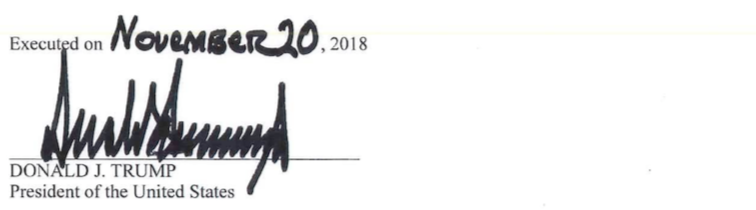
\includegraphics[width=6in]{images/appendix-c-signature.png}%
\end{figure}
